\section{Definición de requisitos y análisis}
\label{sec:definicion_de_requisitos_y_analisis}

\subsection{Definición de requisitos}

% (que se quiere hacer definido de una manera formal)
% descripción del caso de uso

{\color{red} \textbf{!!! TODO}}

\subsection{Arquitectura}

% (Haz un diagrama y luego explicalo, asi te valdrá para la presentación del proyecto)
% diagrama sencillo con la arquitectura: fotos + red neuronal + modelo + móvil

\begin{figure}[H]
	\centering
	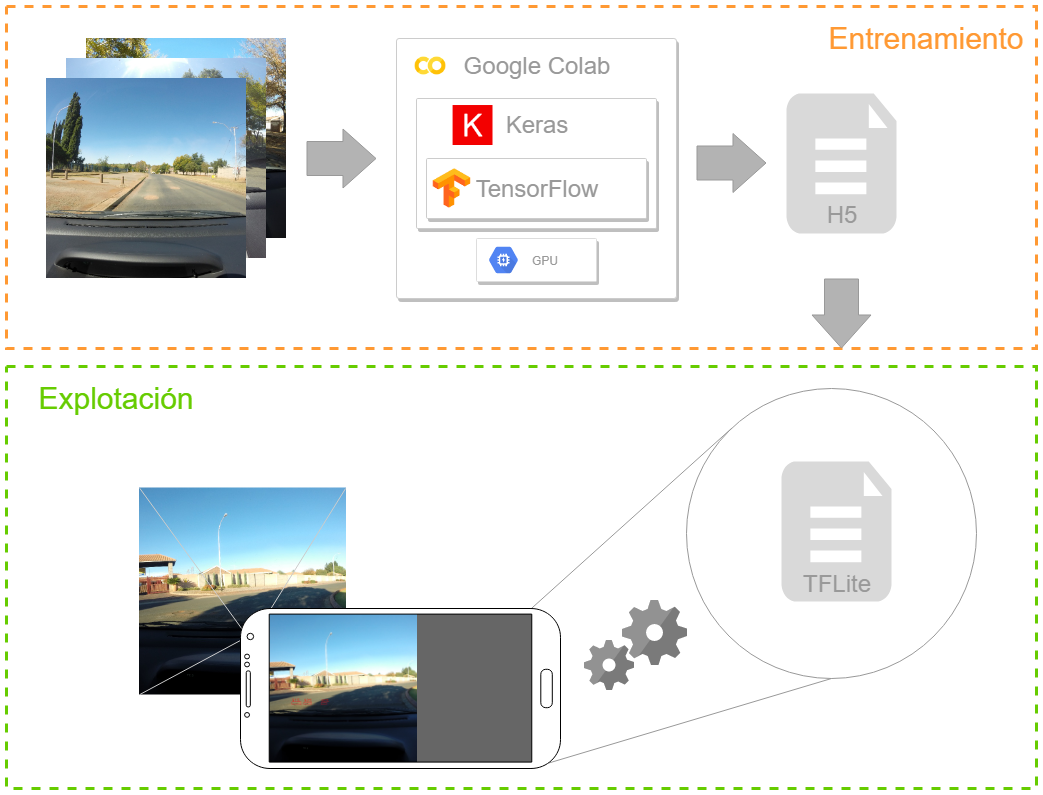
\includegraphics[width=\linewidth]{images/architecture.png}
	\caption{Arquitectura de la solución}
	\label{fig:architecture}
\end{figure}

{\color{red} \textbf{!!! TODO}}

\subsection{Tecnologías}

% (Esto es poco más que enumerar lo que vas a utilizar)
% python, keras, tensorflow, opencv, java, yolo v3, yolo v3 tiny

{\color{red} \textbf{!!! TODO}}